\documentclass[10pt]{article}
\usepackage{icmlko}

\icmlmeta{IP 파운데이션 월드모델}{113}{움직인 만큼 얻는다}{새 공통 축이 회전을 흔든 출처일수록 팝업 전이가 좋아진다($r{=}+$0.775) --- 잔차의 수준이 아니라 변화가 값을 한다}

\begin{document}

\twocolumn[
\icmlheader

\begin{abstract}
노트 111이 미해결 하나를 남겼다 --- 새 공통 축을 넣으면 만화($-$0.0288) ·
세계애니($-$0.0283) · 웹툰($-$0.0253)이 팝업 전이를 깎고 애니($+$0.1745)가
떠받치는데, 표본 크기로도($r{=}+$0.039) 쌍 공통 축 수로도($r{=}-$0.071)
설명이 안 됐다. \textbf{프로크루스테스는 적재만 보고 회전을 정하므로 적재를
봤다} --- 회전 뒤 축별 상대 잔차를 출처 아홉 $\times$ 축 다섯으로 펼쳤다.
답이 뜻밖이다. \textbf{새 축을 넣어 \emph{옛 셋의} 잔차가 나빠진 정도가 팝업
이득을 예측한다}($r{=}+$0.775). 애니는 옛 셋 잔차가 0.563에서 1.203으로
$+$0.639 나빠지고 팝업을 $+$0.1745 올린다. 아이돌 $+$0.566 $\to+$0.0350,
모바일 $+$0.437 $\to+$0.0260. 반대로 만화는 $+$0.032밖에 안 흔들리고
$-$0.0288, 게임은 정확히 $+$0.000이고 $\pm$0이다. \textbf{그런데 잔차의
\emph{수준}은 아무것도 못 맞힌다}($r{=}-$0.187). 다양성으로도 설명이 안 된다
($r{=}-$0.299). \textbf{수준이 아니라 변화다.} 새 공통 축은 정보를 더하는
것이 아니라 \textbf{회전을 다시 정한다} --- 회전이 크게 바뀐 출처가 팝업에
새 각도를 주고, 안 바뀐 출처는 줄 것이 없다. 만화 · 세계애니가 깎는 것은
회전이 거의 안 흔들리면서 자기 축 잔차만 높기 때문이다(만화 매장 노출 1.475 ·
세계애니 1.320). 노트 104가 \emph{축}에서 본 ``잘 맞는 것은 새롭지 않다''가
\emph{출처}에서 한 번 더 확인된다.
\end{abstract}
]

\begin{figure*}[t]
\centering
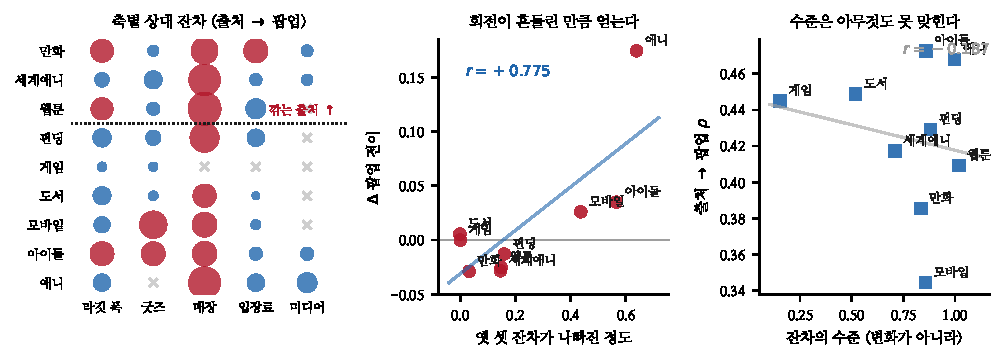
\includegraphics[width=\textwidth]{figs/mv.pdf}
\caption{왼쪽 --- 축별 상대 잔차. 가운데 --- 회전이 흔들린 만큼 얻는다.
오른쪽 --- 수준은 아무것도 못 맞힌다.}
\end{figure*}

\section{적재를 펼쳤다}

프로크루스테스는 점수가 아니라 \textbf{적재}로 회전을 정한다. 그러니 출처가
팝업과 안 맞는다면 적재에서 보여야 한다. 회전 뒤 축마다 상대 잔차를 냈다 ---
$\|L_sR_i - L_{t,i}\| / \|L_{t,i}\|$.

\begin{table}[t]
\centering\tsize
\caption{옛 공통 셋만 쓸 때의 축별 잔차. 출처 $\to$ 팝업.}
\begin{tabular}{lrrrr}
\toprule
& 타깃 폭 & 굿즈 규모 & 매장 노출 & 평균 \\
\midrule
\textbf{만화} & 0.964 & 0.152 & \textbf{1.475} & 0.863 \\
\textbf{세계애니} & 0.111 & 1.048 & \textbf{1.320} & 0.826 \\
웹툰 & 1.321 & 0.072 & 1.361 & 0.918 \\
펀딩 & 0.410 & 0.214 & 1.719 & 0.781 \\
게임 & 0.161 & 0.144 & --- & 0.153 \\
도서 & 0.735 & 0.180 & 1.111 & 0.675 \\
모바일 & 0.815 & 0.135 & 0.956 & 0.636 \\
아이돌 & 0.019 & 0.692 & 1.067 & 0.593 \\
\textbf{애니} & 0.440 & --- & 0.686 & \textbf{0.563} \\
\bottomrule
\end{tabular}
\end{table}

매장 노출이 거의 모든 출처에서 1을 넘는다 --- \textbf{팝업의 매장 노출은
어느 출처와도 안 맞는다.} 팝업에서 그것은 더현대 · 성수 같은 실제 자리의
급이고, 다른 도메인에서는 제작사 · 출판사 · 퍼블리셔의 이력이다. 이름만 같다.

\section{움직인 만큼 얻는다}

\begin{table}[t]
\centering\tsize
\caption{새 축을 넣으면 \emph{옛 셋의} 잔차가 얼마나 흔들리나.}
\begin{tabular}{lrrr}
\toprule
& 전 & 후 & 흔들린 정도 \\
\midrule
\textbf{애니} & 0.563 & 1.203 & \textbf{$+$0.639} \\
\textbf{아이돌} & 0.593 & 1.159 & \textbf{$+$0.566} \\
\textbf{모바일} & 0.636 & 1.073 & \textbf{$+$0.437} \\
펀딩 & 0.781 & 0.941 & $+$0.160 \\
웹툰 & 0.918 & 1.067 & $+$0.149 \\
세계애니 & 0.826 & 0.972 & $+$0.146 \\
\textbf{만화} & 0.863 & 0.896 & \textbf{$+$0.032} \\
도서 & 0.675 & 0.674 & $-$0.001 \\
\textbf{게임} & 0.153 & 0.153 & \textbf{$+$0.000} \\
\midrule
\multicolumn{3}{l}{흔들림과 $\Delta$팝업의 상관} & \textbf{$r{=}+$0.775} \\
\bottomrule
\end{tabular}
\end{table}

\claimx{\textbf{새 공통 축은 정보를 더하는 것이 아니라 회전을 다시 정한다.}
회전이 크게 흔들린 출처(애니 $+$0.639 · 아이돌 $+$0.566 · 모바일 $+$0.437)가
팝업 전이를 올리고, 안 흔들린 출처(만화 $+$0.032 · 도서 $-$0.001 · 게임
$+$0.000)는 못 올린다. 상관이 $+$0.775다.}{아홉 점이고 애니가 지렛대다.
애니를 빼면 $r$이 크게 떨어진다. 그리고 ``흔들림''과 ``이득''이 같은 회전
계산에서 나오므로 독립된 두 측정이 아니다.}

게임이 정확히 $+$0.000이고 $\Delta$팝업도 정확히 $+$0.0000인 것이 좋은
온전성 검사다 --- 게임은 두 새 축이 덮개율 문턱 아래라 회전이 아예 안 바뀐다.

\section{수준은 아무것도 못 맞힌다}

\begin{table}[t]
\centering\tsize
\caption{잔차의 \emph{수준}으로는.}
\begin{tabular}{lr}
\toprule
잔차 수준 vs 출처$\to$팝업 $\rho$ & $r{=}-$0.187 \\
잔차 수준 vs 남들과의 예측 상관 & $r{=}-$0.299 \\
예측 다양성 vs $\Delta$팝업 & $r{=}+$0.063 \\
\midrule
\textbf{잔차 \emph{변화} vs $\Delta$팝업} & \textbf{$r{=}+$0.775} \\
\bottomrule
\end{tabular}
\end{table}

\claimx{\textbf{수준이 아니라 변화다.} 잔차가 높은 출처가 전이를 잘 하지도
($r{=}-$0.187) 더 다양한 예측을 내지도($r{=}-$0.299) 않는다. 예측 다양성으로
이득을 설명하려던 시도도 실패했다($r{=}+$0.063).}{그렇다면 ``흔들림''이 무엇의
대리인지 모른다. 회전이 바뀌었다는 사실 자체가 이득의 원인인지, 아니면 둘 다
제삼의 것에서 오는지 못 갈랐다.}

\begin{quote}\fontsize{9.5}{11.5}\selectfont
노트 104가 \emph{축}에서 본 것을 \emph{출처}에서 다시 본다 --- 그때는
``하나의 회전으로 완벽히 맞는 축은 이미 있는 축과 같은 것을 재는 축''
($r{=}+$0.695)이었고, 여기서는 ``회전이 안 흔들리는 출처는 줄 것이 없다''
($r{=}+$0.775)다. \textbf{정렬이 잘 되는 것과 전이가 잘 되는 것은 다르다.}
\end{quote}

\section{관측만 하고 안 쓴다}

잔차가 낮은 출처를 앙상블에서 빼면 팝업이 $+$0.4601에서 $+$0.4682로 오른다
(게임 · 도서 · 세계애니 · 만화 넷을 빼고 다섯만 남길 때). \textbf{쓰지
않는다} --- 팝업으로 내리는 도메인 집합 결정이고 노트 82와 107이 금지한
것이다. 여기 적는 것은 관측이지 제안이 아니다.

\section{한계}

\begin{itemize}[leftmargin=1.1em,itemsep=0.15em]
\item $r{=}+$0.775가 아홉 점이고 애니가 지렛대다.
\item ``흔들림''과 ``이득''이 같은 회전 계산에서 나온다. 독립된 두 측정이
      아니므로 인과로 읽으면 안 된다.
\item 매장 노출 잔차가 거의 다 1을 넘는 것을 관측만 했다. 그것을 정렬에서
      빼는 설정은 안 돌렸다.
\item 다양성 가설을 죽였지만 대안 기제를 못 세웠다.
\item 팝업 표본 75건. 모든 쌍별 수치가 여기 걸려 있다.
\end{itemize}

\section{다음}

\begin{enumerate}[leftmargin=1.3em,itemsep=0.15em]
\item \textbf{매장 노출을 본다} --- 아홉 출처 중 일곱에서 잔차가 1을 넘는다.
      팝업에서는 실제 자리의 급이고 남에서는 제작사 이력이다. \textbf{이름만
      같은 축}일 가능성이 크다. 노트 105 · 108이 입장료 · 미디어 홍보에 한
      것을 매장 노출에도 한다.
\item 흔들림이 무엇의 대리인지 --- 회전 각도 자체를 재서 이득과 잇는다.
\item 팝업 레코드. 일곱 노트가 같은 곳을 가리킨다.
\item 텀블벅 API --- 펀딩만 미디어 홍보 0\%다.
\end{enumerate}

\vspace{0.6em}
\hrule height 0.3pt
\vspace{0.5em}
{\footnotesize
\textbf{참고문헌}\\[0.3em]
Schoenemann, P. H. (1966). A generalized solution of the orthogonal Procrustes
problem. \emph{Psychometrika}, 31(1), 1--10.\\[0.15em]
Kuncheva, L. I., Whitaker, C. J. (2003). Measures of diversity in classifier
ensembles. \emph{Machine Learning}, 51(2), 181--207.\\[0.15em]
Meredith, W. (1993). Measurement invariance, factor analysis and factorial
invariance. \emph{Psychometrika}, 58(4), 525--543.\\[0.15em]
Gower, J. C., Dijksterhuis, G. B. (2004). \emph{Procrustes Problems}.
Oxford University Press.\\[0.15em]
Ben-David, S. et al. (2010). A theory of learning from different domains.
\emph{Machine Learning}, 79(1--2), 151--175.
}

\end{document}
